% !TEX program = xelatex
\documentclass[
  10pt,
  twoside,
  openany,
  b5paper, % 以上均为 ctexbook 提供的文类选项
  colorscheme = basic, % 请根据需要选择或定制配色方案
]{qyxf-book}
\usepackage{pdfpages}
\usepackage[contents = 钱院学辅, scale = 15, color = black, angle = 50, opacity = .10]{background}


\title{复变函数与积分变换思维导图}
\subtitle{Mind Map of Complex Analysis and Integral Transformation}  % 可选
\author{电气钱91班谢佳润}
\date{2021 年 1 月 6 日}
%\typo{AlphaGo}  % 排版人员信息,选填

% 定制元信息
\org{\Large\textit{钱学森书院学业辅导中心}\\\textsc{Qian Xuesen College Academic Counseling Center}}
\footorg{\textsc{Qian Yuan Xue Fu}}
\cover{
	\begin{tikzpicture}[remember picture, overlay]
		\begin{pgfonlayer}{background}
			\node at ($(current page.east)+(0in,0in)$){
				
\includegraphics[width=.8\textwidth]{cover.png} };
		\end{pgfonlayer}
	\end{tikzpicture}
}
\license{}  % 清空许可证信息

% 调整封面标题大小
\renewcommand{\titlefont}{\Huge\bfseries}
\renewcommand{\subtitlefont}{\LARGE\itshape}

\begin{document}

\maketitle

\chapter*{前言}
\thispagestyle{empty}

《复变函数》几乎是所有理工科学生的必修课,可以说只要你的专业与“电”相关,你或早或晚都要接触这门课程。相信经过了一学期的学习,各位同学都会对这门课程有着自己的感悟与理解。可能有些同学已经发现这门课程作为工科生的一项“工具”,解题的技巧性并没有那么的强,更多的则是需要记忆并熟练运用样式繁多且容易混淆的公式,而这也恰恰成为一些同学(包括笔者)学习过程中的一些阻碍。所以为了方便记忆同时避免遗漏,笔者在学习之余,将书本上的一些知识要点与公式进行整理,以思维导图的形式呈现出来以理解与复习。

但事实上我并不愿称这一份资料为思维导图,因为其中有些内容过于冗杂甚至可能无用,丝毫没有体现出思维导图的简洁之美。可毕竟笔者能力有限,没有想到一些更好的解决办法,最后只能靠最原始的堆叠与罗列,将知识要点和常用公式呈现出来,并稍微做一些整理,让读者在阅读时能够更快的检索到需要的信息,也方便读者更加系统的去记忆公式。

同时我也相信这份资料对于很多同学其实是无用的,因为一方面其中所有的内容都可以在书上相应位置找到,我做的工作只不过是将它们提取出来,整理到一起;另一方面这些同学也早已根据自己的理解建立起适合自己的学习体系,不需要类似这种资料的辅助。所以大家使用时各取所需就好,而这一份资料的受众群体,也正是那些目前仍需要依靠外部资料协助来进一步掌握知识的同学。另外笔者只是一名普通的同级工科生,能力有限,所以编纂的时候难免会有些错误与遗漏之处,任何与资料内容有关的建设性批评与建议,都欢迎大家积极提出,希望这份资料能够给大家提供适当的帮助,谢谢各位同学!

最后还有一些闲话想要说,很多同学可能会疑惑为什么我们要去学习《复变函数》这门课程,刚开始的时候我也同样如此。但慢慢的在自己学习、查阅资料以及和学长交流的过程中,我逐渐意识到这门课的重要性,借用知乎上一位前辈的回答说:

“复变函数是电的五线谱”

《复变函数》作为未来很多专业课学习的基础,其重要程度,不言而喻。所以希望同学们,尤其是专业与“电”相关的同学,要对这门课程足够重视起来,在复习的过程中也要多一些自己的理解与思考,不要将自己的思想单单的拘泥于记忆公式本身,更多的是要跳脱出公式,真正理解公式背后的意义与使用的精髓所在。

\rightline{——电气钱91班\ 谢佳润} 


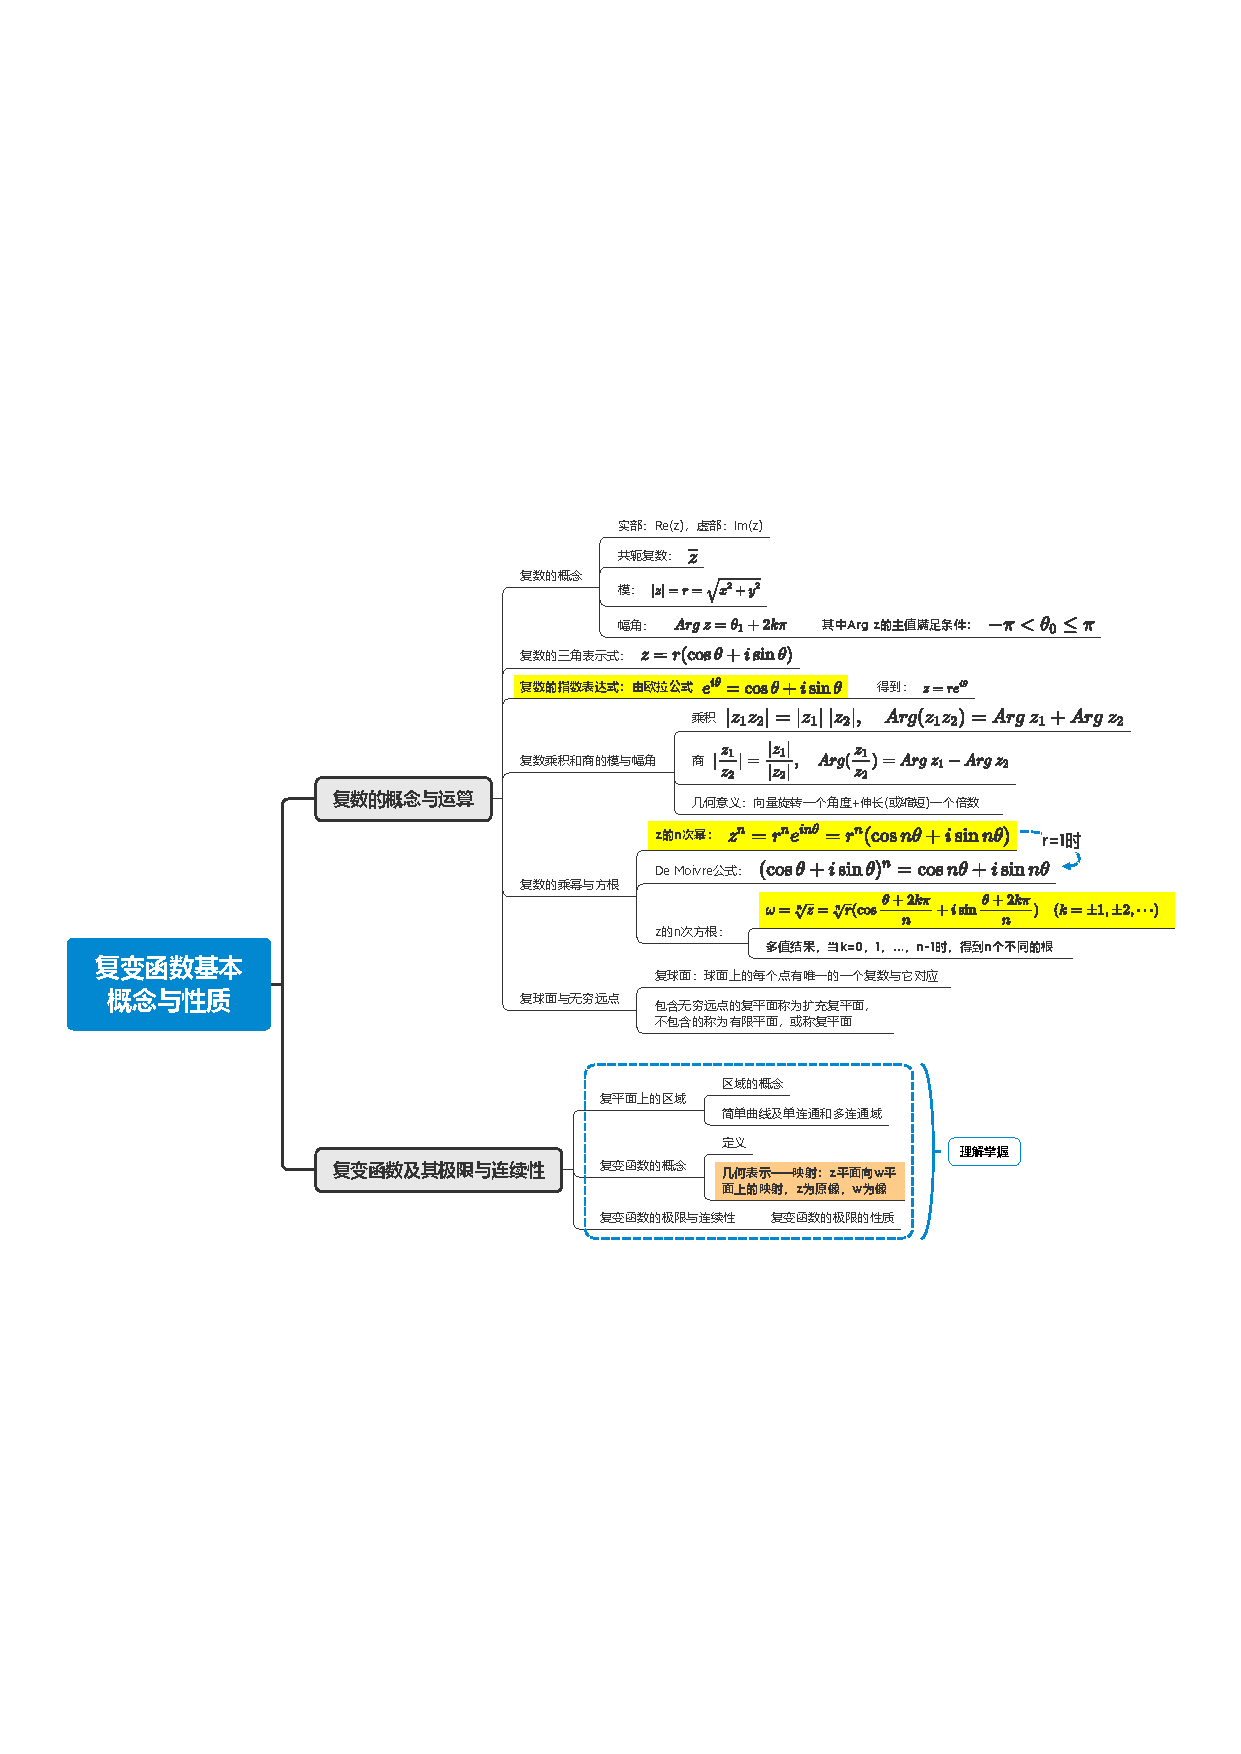
\includepdf[pages = - ]{content.pdf}


\end{document}